\documentclass[tikz,border=10pt]{standalone}
\usetikzlibrary{shapes}
\usetikzlibrary{arrows}
\usetikzlibrary{positioning}
\begin{document} 

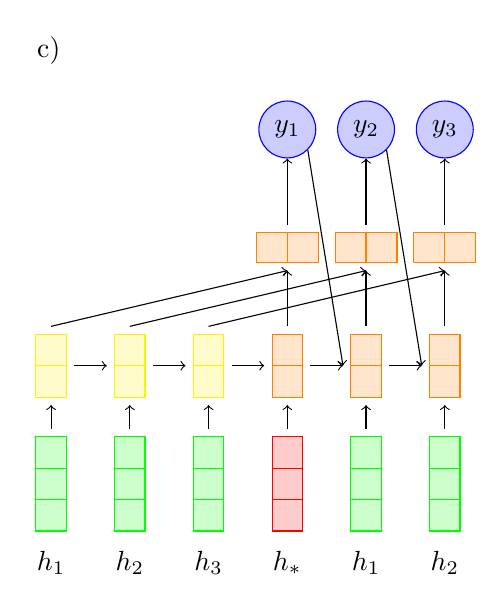
\begin{tikzpicture}[
  hid/.style 2 args={
    rectangle split,
    draw=#2,
    rectangle split parts=#1,
    fill=#2!20,
    outer sep=1mm},
  mlp/.style 2 args={
    rectangle split,
    rectangle split horizontal,
    draw=#2,
    rectangle split parts=#1,
    fill=#2!20,
    outer sep=1mm}
]

  \node [anchor=west] (label) at (.7, 4.5) {c)};
 \foreach \i [count=\step from 1] in {$h_1$, $h_2$, $h_3$, $h_*$, $h_1$, $h_2$}
    \node (i\step) at (1*\step, -2) {\i};
  % draw embedding and hidden layers for text input
  \foreach \step in {1,...,3} {
    \node[hid={3}{green}] (e\step) at (1*\step, -1) {};    
    %\draw[->] (i\step.north) -> (e\step.south);
  }
    \node[hid={3}{red}] (e4) at (1*4, -1) {};    
  \foreach \step in {5,...,6} {
    \node[hid={3}{green}] (e\step) at (1*\step, -1) {};    
    %\draw[->] (i\step.north) -> (e\step.south);
  }

  \foreach \step in {1,...,3} {
    \node[hid={2}{yellow}] (h_f_\step) at (1 *\step, .5) {};    
%    \node[hid={2}{yellow}] (h_r_\step) at (.25 + .9 *\step, 1.25) {};    
    \draw[->] (e\step.north) -> (h_f_\step.south);
%    \draw[->] (e\step.north) -> (h_r_\step.south);
%    \node[mlp={2}{yellow}] (h_\step) at (.9 *\step, 2.5) {};    
%    \node[circle, draw=blue, fill=blue!20] (y_\step) at (.9 *\step, 3.75) {$y_\step$};    
%    \draw[->] (h_\step.north) -> (y_\step.south);
%    \draw[->] (h_f_\step.north) -> (h_\step.south);
%    \draw[->] (h_r_\step.north) -> (h_\step.south);
  }
  \foreach \step in {4,...,6} {
    \node[hid={2}{orange}] (h_f_\step) at (1 *\step, .5) {};    
    \node[mlp={2}{orange}] (g_f_\step) at (1 *\step, 2) {};    
    \draw[->] (e\step.north) -> (h_f_\step.south);
    
 }
  \foreach \step in {1,...,3} {
    \node[circle, draw=blue, fill=blue!20] (y_\step) at (3 + 1 *\step, 3.5) {$y_\step$};    
 }
    \draw[->] (y_1.south east) -> (h_f_5.west);
    \draw[->] (y_2.south east) -> (h_f_6.west);
    \draw[->] (h_f_4.north) -> (g_f_4.south);
    \draw[->] (g_f_4.north) -> (y_1.south);
    \draw[->] (h_f_5.north) -> (g_f_5.south);
    \draw[->] (g_f_5.north) -> (y_2.south);
    \draw[->] (h_f_6.north) -> (g_f_6.south);
    \draw[->] (g_f_6.north) -> (y_3.south);
 \foreach \step/\steppp in {1/2, 2/3, 3/4, 4/5, 5/6} {
   
    \draw[->] (h_f_\step.east) -> (h_f_\steppp.west);
    %\draw[->] (h_r_\steppp.west) -> (h_r_\step.east);
  }
    \draw[->] (h_f_1.north) -> (g_f_4.south);
    \draw[->] (h_f_2.north) -> (g_f_5.south);
    \draw[->] (h_f_3.north) -> (g_f_6.south);



\end{tikzpicture}







\end{document}
